\section{Anforderungsanalyse}

\subsection{Systembeschreibung}

    Die zu entwickelnde Anwendung verfolgt einen datengetriebenen Ansatz. Die Daten müssen erhoben werden um diese dann über ein Webfrontend darstellbar zu machen.  Die interessierten Benutzer  können sich über die Web Präsenz die letzte Position der Bojen auf einer Karte ansehen. Durch einen Klick auf die Darstellung einer Messboje erhalten sie zudem Informationen und eine Darstellung der von dieser Messstation gemessenen Messwerte.
    
    

% BEGIN ermittlung  Anforderungen 
    \subsection{Ermittlung der Anforderungen}
    
    Ausgehend von einem ersten Prototypen  und über User-Stories wurden einige Use-Cases entwickelt \footnote{Siehe Abbildung \ref{fig:use_case}: \nameref{fig:use_case}}.  Hierbei wurden die zwei Klassen "`Benutzende"' \textbf{(B)} und "`Administrierende"'  \textbf{(A)} mit den ihnen zugehörigen Anwendungsfällen herausgearbeitet. 
    
    \begin{figure}[h!]
        \centering
        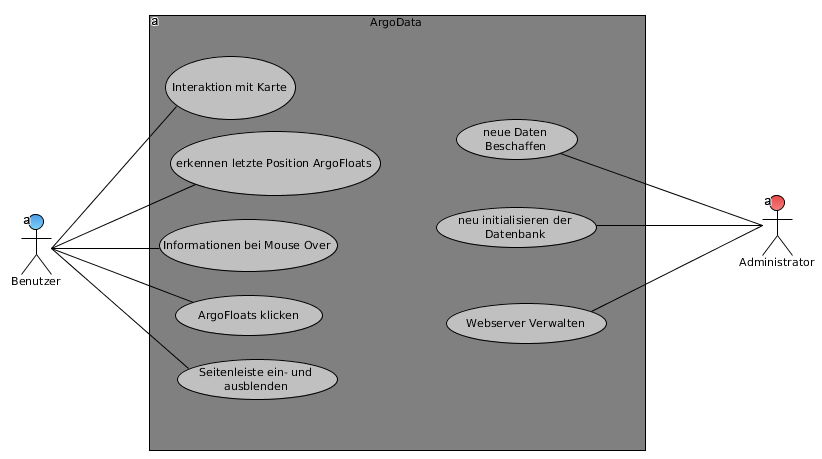
\includegraphics[width=0.8\textwidth]{pix/use-case.png}
        \caption{Use case Diagramm der Anforderungen}
        \label{fig:use_case}
    \end{figure}
    
    Anhand des so vorliegenden Modells wurde ein Abhängigkeitsgraph ausgearbeitet.\footnote{Siehe Abbildung \ref{fig:graph_anforderungen}: \nameref{fig:graph_anforderungen}}.  Dieser beschreibt die Anforderungen und deren Abhängikeiten anhand eines gerichteten Graphen. Mit hilfe dieser Darstellung konnten die Anforderungen noch feiner ausgearbeitet und um Definitionslücken erweitert werden.  
    
    \begin{figure}[h!]
    \centering
    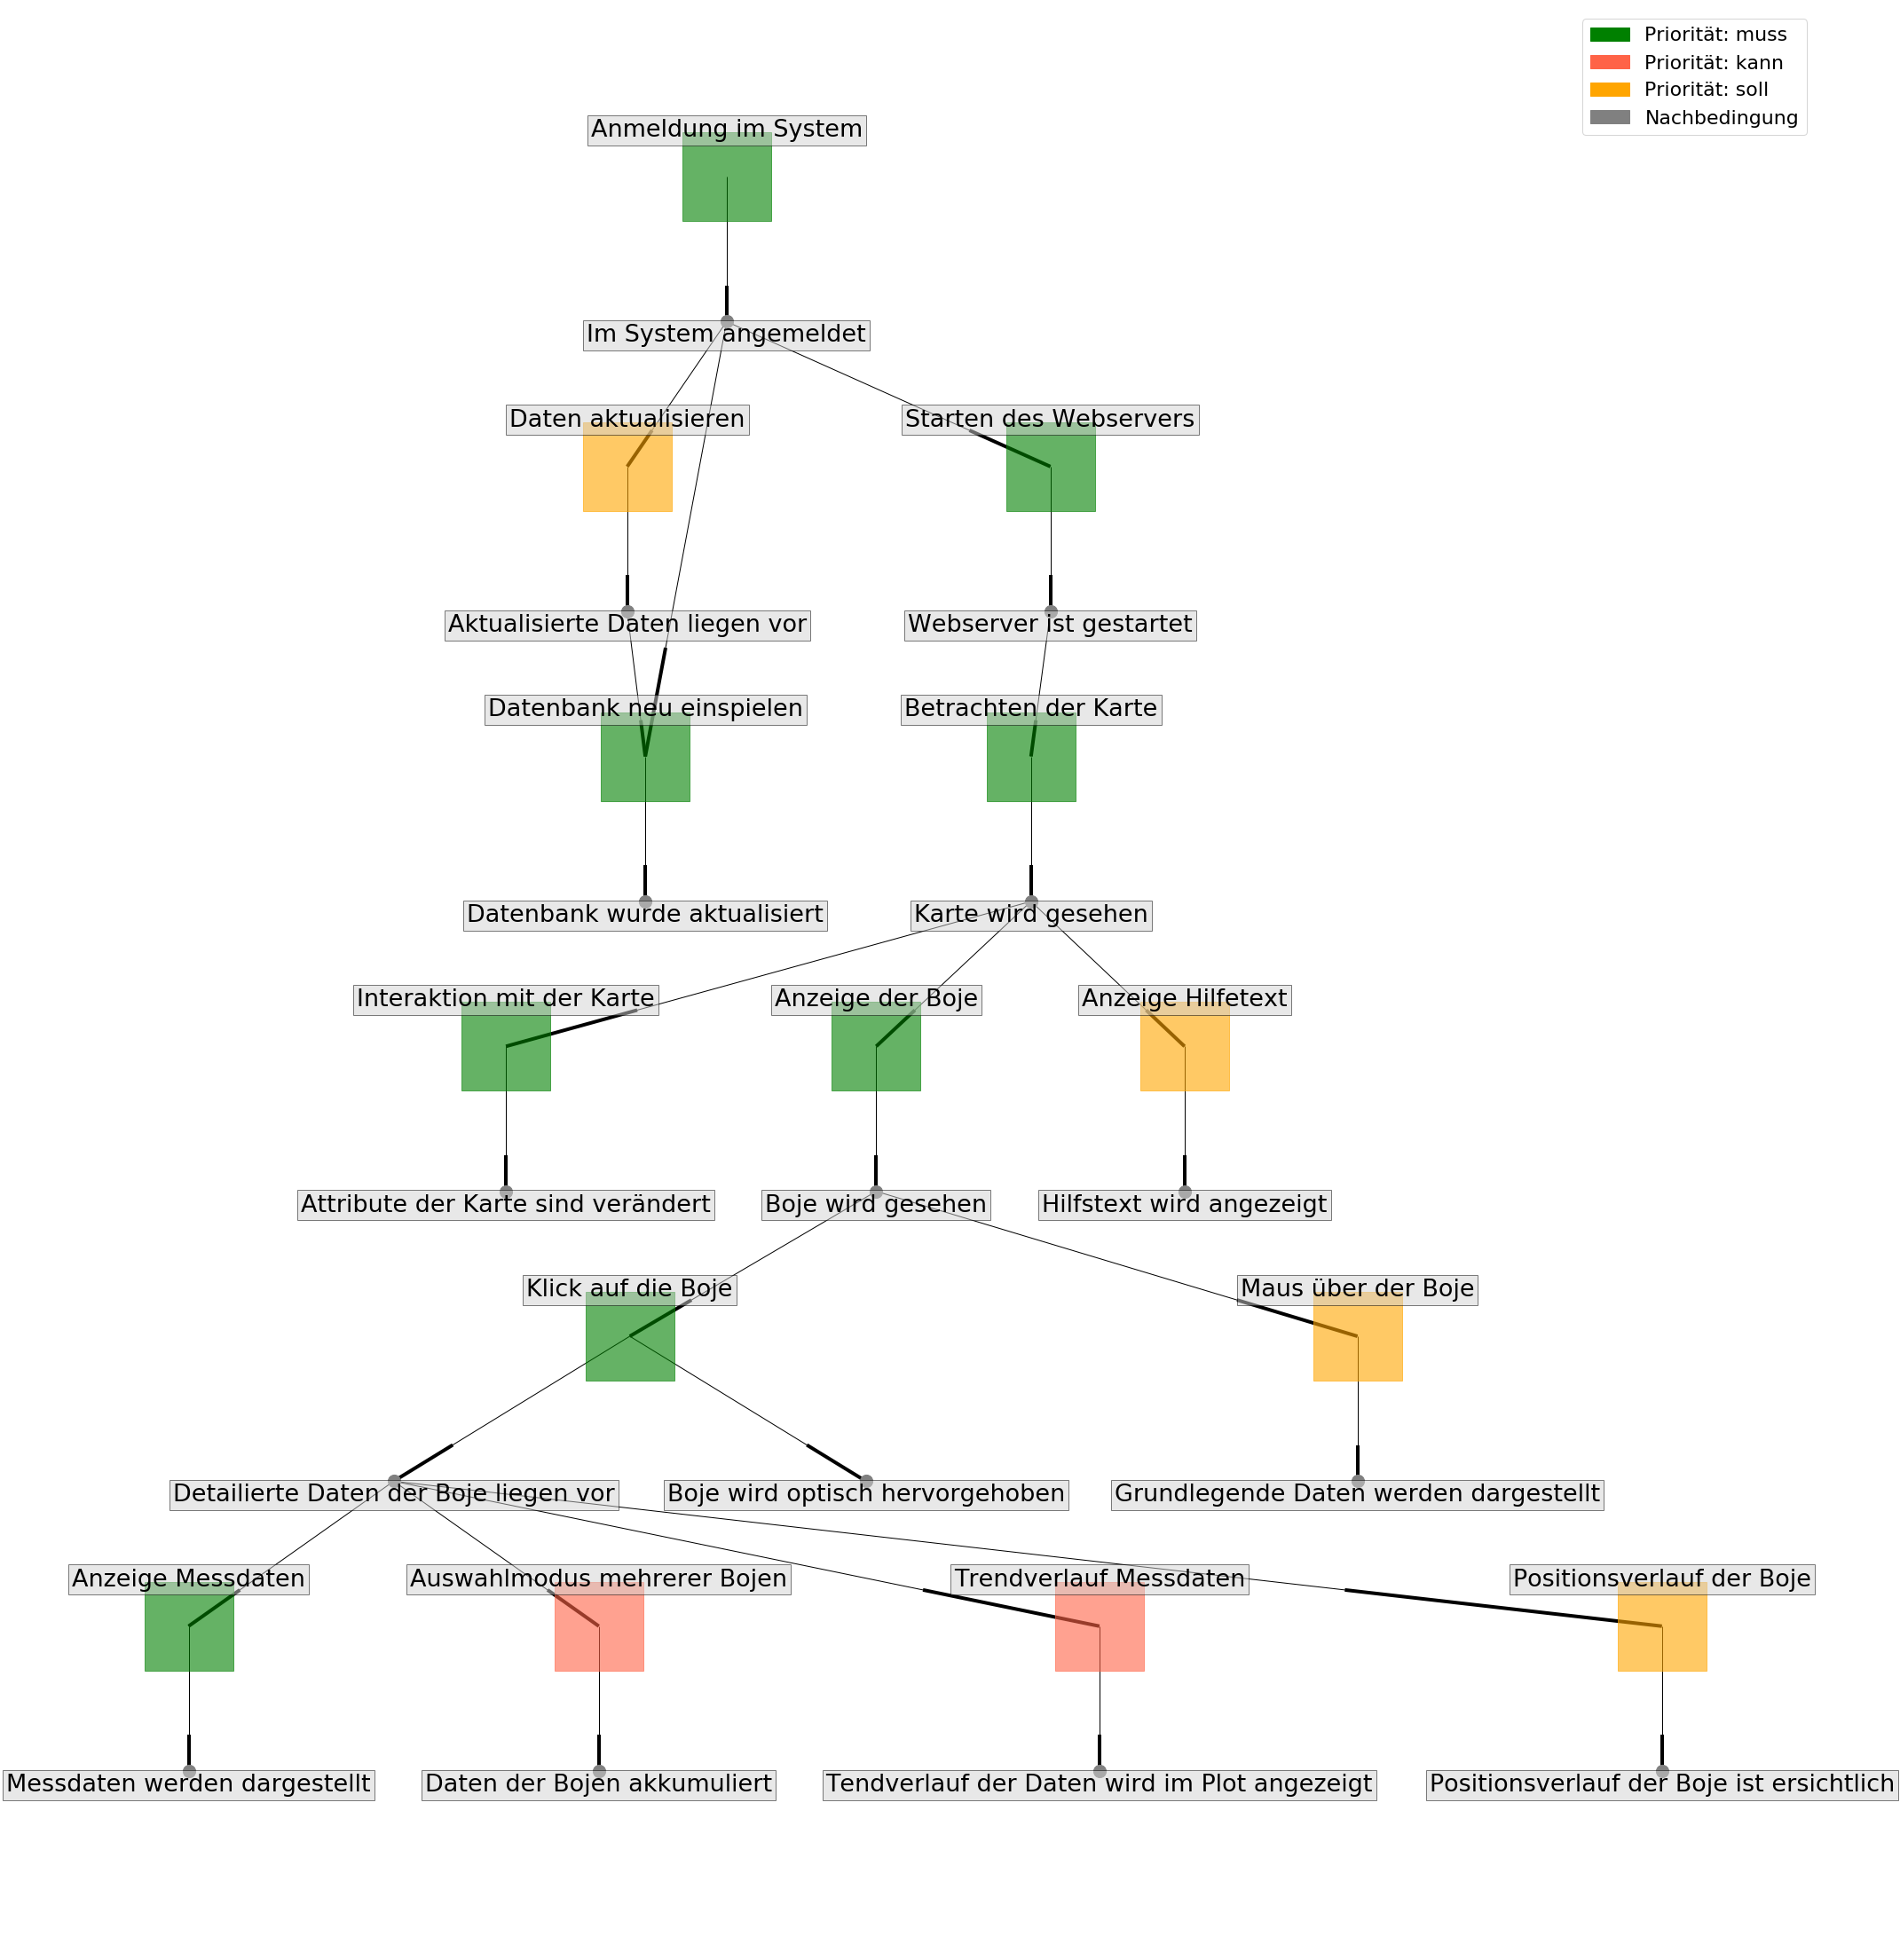
\includegraphics[width=\textwidth]{pix/graph_anforderungen.png}
    % graph_anforderungen.png: 1208x850 px, 72dpi, 42.63x29.99 cm, bb=0 0 1208 850
    \caption{Anforderungen und ihre Abhängigkeiten als gerichteter Graph}
    \label{fig:graph_anforderungen}
    \end{figure}
    
% END 
     
% BEGIN Beschreibung  funktionale Anforderungen
    \subsection{Funktionale Anforderungen}
    
    \subsubsection{Anwendende Perspektive}
    
    Die benutzenden erwarten die Darstellung einer Webapplikatin wenn diese die ihr zugehörige URL öffnen. Die Webseite soll über eine Kartenapplikation die Grenzen der Ozeane und der umliegenden Kontinente ersichtlich machen.  Eine genauere Darstellung von Landmarkern wie Straßen, Städte oder Gebirge ist für den Aussagewert der Applikation nicht erforderlich. Die Kartendarstellung soll außerdem über Interaktionsmöglichkeiten, wie dem Einstellen der Zoomstufe, sowie des ausgewählten Kartenbereichs, verfügen.
    
    Über den Kartendienst sind außerdem die letzte Position jeder Messboje aus dem Datensatz ersichtlich. Über Farbcodes wird der Status der Boje auf den ersten Blick erfahrbar gemacht. Um Streuung und Verdichtung an spezifischen Orten ersichtlich zu halten, werden alle Messstationen des angezeigten Kartenausschnittes dargestellt. Es erfolgt keine Zusammenfassung oder Ausblendung der Messstationen.
    
    Wird die Maus über eine Boje geführt, so ist es sinnvoll hier bereits grundlegende Daten der Messstation darzustellen um eine Identifikation des jeweiligen Datensatzes zu ermöglichen.
    
    Ein Mausklick auf die schematische Darstellung der Boje soll spezifischere Daten der Boje anzeigen. Dazu soll in einem separierten Darstellungsfeld, der Verlauf der Messdaten, sowie einiger weiterer sinnvoller Werte der jeweiligen Messstation angezeigt werden. Es ist sinnvoll, wenn dieser Bereich je nach Wunsch des Benutzenden zu- und wieder abgestellt werden kann. 
    
    
    \subsubsection{Administrative Perspektive}
    
    Um die Inhalte zu erstellen, werden auf Administrativer Sicht keine Journalistischen Tätigkeiten erwartet. Durch den Datengetriebenen Ansatz der Applikation müssen für das Erstellen der Inhalte keine Webmasken wie Texteingabefelder zur Verfügung gestellt werden. Vielmehr ist es hier sinnvoll, die hier benötigten Werkzeuge als Skripte zur Verfügung zu stellen, um die Administrativen Aufgaben über die Kommandozeile ausführen zu können. 
    
    Administrierende erwarten vom System dass sie neue Daten  in die Datenbank überführen können. Hierbei ist es notwendig, dass die Datensätze des Argo Programms ausgelesen und in ein für die Datenbank aufbereitetes Format überführt werden. 
    
    Es wäre sinnvoll, die Aggregation der POIs ebenfalls über einen Programmablauf zu modellieren.  In diesem Schritt müssten die Daten von der Webpräsenz des gooc heruntergeladen und an einem Ort entpackt werden. Zusätzlich müsste darauf geachtet werden, die Daten wieder zu entfernen, nachdem diese in die Datenbank des Systems überführt worden ist.
    
    Der Prozess der Beschaffung und Aktualisierung der Daten kann bis hin zur Vollautomatisierung abgebildet werden. 
% END 
    

% BEGIN Beschreibung  nicht-funktionale Anforderungen


\subsection{Nicht-Funktionale Anforderungen}
    
    \subsubsection{Anwendende Perspektive}
        Für die Benutzenden ist die Usability der wichtigste Aspekt. Die Benutzungsmuster müssen klar ersichtlich und intuitiv erfahrbar sein. Die Darstellung der Applikation soll einfach und schlicht gehalten werden und dem gewohnten Erscheinen modernen Web Applikationen entsprechen. 
        
        Es soll darauf Wert gelegt werden, die Daten möglichst schnell nach der Interaktion zu Anzeige zu bringen, da das Warten auf Webapplikationen mit Frust verbunden ist, und eine hohe Absprungrate zur Folge hätte.
        
        
    \subsubsection{Administrative Perspektive}
        Für die Aggregation der Daten ist die Sicherheit ein zentraler Aspekt. Dies umfasst sowie Aspekte von Authentifizierung und Autorisierung der Rolle der Datenaggregation als auch eine Sicherheit um die Integrität der Heruntergeladenen Daten.
    
% END 

% BEGIN Auswahl der Daten
\subsection{Benötigte Daten}

Um die Darstellung zu vereinfachen und die Kommunikation mit der Datenbank zu beschleunigen, ist im ersten Schritt eine Auswahl aus den Daten der Argo-Bojen vorzunehmen. Hierbei soll darauf geachtet werden, nur diejenigen Daten zu verwenden, welche für die Erbringung des Dienstes notwendig sind.

Aus diesem Grund findet sich im Folgenden eine Auswahl aus dem Datenkatalog \footnote{Siehe Quelle \cite{ArgoUserManual} S. 19 ff.} von Argo mit der jeweiligen Begründung:

\begin{center}
    \begin{tabular}{ | l | p{4cm} |p{6cm} |}
    \hline
    \textbf{Datenfeld} & \textbf{Beschreibung} & \textbf{Wird verwendet weil} \\\hline
   
    PLATFORM\_NUMBER 
        & Eindeutige Identifikationsnummer einer einer Messstation
        & Wird benötigt um Messprofile eindeutig der Plattform zuordnen zu können. \\\hline 
    
    CYCLE\_NUMBER 
        & Fortlaufende und innerhalb einer Messboje eindeutige Identifikationsnummer eines Messprofils
        & Dieser Wert wird benötigt, um Messungen eindeutig zuordnen zu können. \\\hline
    
    JULD
        & In Julian Date codierter Zeitpunkt der Übertragung (Begin oder ende?) einer Messung
        & Der Zeitpunkt wird benötigt um die Messungen in einen Zeitlichen Kontext zu stellen. \\\hline
        
    N\_PARAM
        & Anzahl der Messsensoren. 
        & Durch diesen Wert lässt sich die Anzahl der Sensoren ableiten. \\\hline
        
    LATITUDE \& LONGITUDE
        & Die Positionsdaten einer Messung zum Zeitpunkt der Übetragung der Werte.
        & Dies ist ein essentieller Parameter um die Messungen in einen lokalen Zusammenhang zu stellen. \\\hline
        
    PRES
        & Messvektor des Wasserdrucks
        & Durch diesen Messwert lässt sich die Dichte der überliegenden Wassersäule herleiten. \\\hline
        
    TEMP
        & Messvektor der Wassertemperaturen 
        &  Die Temperatur des umliegenden Wassers ist einer der zentralen Messwerte. Durch diesen Messwert und seinen Trend lässt sich der Globale Klimawandel anschaulich darstellen.  \\\hline
        
    PSAL
        & Messvektoren des Salzgehaltes
        & Ein weiterer Parameter, um die Auswirkungen des Klimawandels zu erfahren. Durch das Schmelzen der großen Eissschelfs an den Polen des Planeten ist eine Verringerung des Salzgehaltes der meere zu erwarten. \\\hline
    \end{tabular}
\end{center}

 

%TODO Der kleine Satz möchte aus den Untiefen der Schachtelsätze abgeholt und verbessert werden
\paragraph{Vereinfachung der Messdaten}
Die verwendeten Messwerte PRES, TEMP und PSAL eines Messprofils liegen in Vektorieller Form vor. Für die Darstellung über einen univariaten Graphen wird nur ein skalarer Wert pro Messprofil benötigt. Die Daten sollen zusammengefasst werden, bevor diese in die Datenstruktur überführt werden um die größe der Daten zu verringern. 
%TODO Implementierung welcher Algorithmus zurzusammenfassung 
 
% END 

% BEGIN technische Anforderungen
\subsection{Technische Anforderungen  }

\subsubsection{Verwendete Programmiersprachen}

Die Darstellung der Webapplikation wird mit HTML und Javascript umgesetzt werden. Diese Sprachen gelten in der Entwicklung von Webseiten als Standard und werden von den gängigen Browsern unterstützt.

Die weiteren teile der Applikation soll mit einer Sprache entwickelt werden, die alle benötigten Teilbereiche umsetzen kann.

Das \textbf{Öffnen der netCDF} Dateien und die numerische Berechnung kann mit C, Java/Scala, R und Python erfolgen. Insbesondere die beiden letzten sind in der Datenverarbeitung und Numerik als etablierte Werkzeuge zu sehen.

Die Darstellung der Seite soll durch ein Webframework unterstützt werden. Hier gibt es in beinahe allen Hochsprachen entsprechende Werkzeuge. Wählt man aus der Problemstellung der numerischen Verarbeitung R und Python heraus, so ist die Auswahl der geläufigen Webframeworks bei Python höher anzusehen. Diese Sprache besitzt eine große Anzahl von Bibliotheken für die Anbindung von Datenbanken, sowie einige etablierte Bibliotheken für die Schaffung von Webapplikationen.  

Python besitzt in Hinsicht auf Laufzeitkosten und einer nicht strikten Typisierung einige Nachteile gegenüber Sprachen wie C und Java. In Hinsicht die auf Auswahl von Programmbibliotheken, sowie der numerischen Berechnung besitzt die Sprache aber Vorteile und wird deswegen hier für die Implementierung genutzt.



\subsubsection{Server}

Für die Laufzeitumgebung der Applikation wird ein GNU/Linux eingesetzt werden. Die Software wird so entwickelt das sie unter den gängigen Distributionen lauffähig sein wird. Hier wird sich aber für Debian stable als Betriebssystem udn Laufzeitumgebung entschieden.


% ?? FOLGENDE ZEILEN NOCH VERWENDEN ??
% 
% Als Laufzeitumgebung ist ein GNU/Linux System einzusetzen. Die Aktualität der Pakete ist nicht von hoher Priorität, vielmehr sollten die bereitgestellten Programme gut getestet und stabil sein. In diesem Kontext gibt es zwei große Distributionen.
% 
% \begin{description}
%  \item [RHEL / centOS] Eine Kommerzielle Distribution und ihr freier Ableger. Von Vorteil sind hier der gute kommerzielle Support. In der Grundausstattung liefert Red Hat nur eine sehr beschränkte Paketauswahl.
%  \item [Debian] Diese Distribution besitzt eine große Community, die aktiv arbeitet und guten Support bietet. Die Paketauswahl ist sehr groß und sicherheitspatches werden schnell bereitgestellt. Mit apt und dpkg besitzt Debian einen exelenten Paketmanager. 
% \end{description}
% 
% Unter diesen Gesichtspunkten erscheint Debian als die geeignetste Distribution für dieses Projekt.

\subsubsection{Webframework}

Für Python gibt es eine große Anzahl an Werkzeugen für die Entwicklung von Webseiten. Hier werden exemplarisch 3 herausgegriffen und für die hier vorliegende Aufgabe bewertet.

\begin{description}
 \item [Django] wird beworben als \texttt{The web framework for perfectionists with dead\-lines}. Es wurde 2005 unter einer BSD Lizenz released und entwicklet, die News-Seite des \textit{Lawrence Journal-World} umzusetzen und zu verwalten. Django ist ein etabliertes und häufig verwendetes Webframework. Es ist dynamisch einsetzbar und für eine große Anzahl von Anwendungen verwendbar. Die Bibliothek ist außerdem durch Module erweiterbar. Die Software folgt dem "`\textit{batteries included}"' Ansatz und liefert in der Grundausstattung bereits alles nötige mit, um eine Webseite inklusive Login und Eingabemasken für journalistische Tätigkeiten auszubauen.
 
 \item [Flask] ist ein sogenanntes Micro-Framework. es verwendet die Toolsammlung \textit{Werkzeug} um Webseiten darstellbar zu machen. Das Farmework folgt dem KISS Ansatz und liefert im Grundumfang nur diejenigen Werkzeuge, die man für die Verwaltung von einfachen Webseiten benötigt. Die Software lässt sich über Module erweitern. Einzelne Teilprojekte von Applikationen lassen sich in sogenannte Blueprints modularisieren. 
 
 \item [Falcon] ist ebenso als Microfarmework zu sehen. Es wurde insbesondere in Hinblick auf Geschwindigkeit entwickelt. Das Framework erlaubt requests asynchron zu verarbeiten und lässt die auf Geschwindigkeit spezialisierte Python-Laufzeitumgebung pypy zu. Falcon ist ein relativ neues Framework und erfährt in letzter zeit zur Schaffung von REST-APIs immer mehr Aufmerksamkeit. Es ist aber auch möglich, mit diesem Framework Webapplikationen mit einer Anzeige über HTML-Elementen zu gestalten. 
\end{description}

In dieser Applikation wird die Schaffung von Journalistischen und redaktionellen Inhalten eine sehr geringe Rolle spielen. Unter diesem Gesichtspunkt ist die Frage der Komplexität der verwendeten Software zu klären. (..) Unter diesem Aspekt erscheint Django nicht als die ideale Wahl.

Flask und Falcon verfogen beide den Ansatz eines Microframeworks. Die Laufzeitgeschwindigkeit des Controllers erscheint an dieser Stelle nicht als limitierender Faktor der Applikation. Zwar wäre es wünschenswert, die Datenbeschaffung der Webapplikation bereits im Backend asynchron zu erledigen, doch überwiegt das breitere Spektrum an Modulen und Dokumentationen für die Webentwicklung von Flask.

Damit erscheint Flask als das geeignetste Werkzeug für diese Aufgabe.


\subsubsection{Datenbank}

Das DBMS soll über Schnittstellen in den Sourcecode des Programmes eingebunden werden. Die datenbank soll einem relationalen schema folgen. Die Verwendung sollte kostenfrei möglich sein und die benötigte Software über die Quellen des betriebssystems verfügbar sein. 

In dieser Applikation wurde sich für die Verwendung von PostgreSQL entschieden. Als Object-Realational-Mapper steht für Python SQLAlchemy zur verfügung.


% END  
